\documentclass[11pt]{article}

\usepackage[margin=1in, headheight=14.5pt]{geometry}
\usepackage{amsfonts, amsmath, amssymb}
\usepackage{enumitem}
\usepackage[none]{hyphenat}
\usepackage{fancyhdr}
\usepackage[spanish, es-noshorthands]{babel}
\usepackage[spanish, calc]{datetime2}
\usepackage{fmtcount}
\usepackage{graphicx}
\usepackage{float}
\usepackage[nottoc, notlot, notlof]{tocbibind}
\usepackage{tocloft}
\usepackage[utf8]{inputenc}
\usepackage{parskip}
\usepackage{xcolor}
\usepackage{cancel}
\usepackage{textcomp}
\usepackage{pgfplots}
\usepackage{tikz}
\usetikzlibrary{shapes.misc}
\usepackage{polynom}
\usetikzlibrary{datavisualization}
\usetikzlibrary{datavisualization.formats.functions}
\pgfplotsset{compat=1.15}
\usepackage{mathrsfs}
\usetikzlibrary{arrows}

\newcommand{\dropsign}[1]{\smash{\llap{\raisebox{-.5\normalbaselineskip}{$#1$\hspace{2\arraycolsep}}}}}%


\parindent 0ex

\pgfplotsset{width=10cm,compat=1.9}

\def\imj{\mathrm{j}}
\def\sen{\mathrm{sen}}

\newcommand{\lapl}[1]{\mathscr{L} \left\lbrace {#1} \right\rbrace}
\newcommand{\ilapl}[1]{\mathscr{L}^{-1} \left\lbrace {#1} \right\rbrace}

\renewcommand\cftsecleader{\cftdotfill{\cftdotsep}}
\renewcommand{\baselinestretch}{1.1}
\newcommand*\circled[1]{\tikz[baseline=(char.base)]{
		\node[shape=circle,draw,inner sep=2pt] (char) {#1};}}
	
\newcommand{\highlight}[2]{\colorbox{#1}{$\displaystyle #2$}}

\graphicspath{{\ProjectRoot/commons/img/}}

\newcommand*{\ProjectRoot}{../../matematica-superior}


\begin{document}
		
	\begin{titlepage}
		\begin{center}
			\vspace*{0.5cm}
			\Large{\textbf{Universidad Tecnológica Nacional}}\\
			\Large{\textbf{Facultad Regional Buenos Aires}}\\
			\begin{center}
				
\includegraphics[scale=0.4]{logoutn.png}
			\end{center}
			\vfill
			\line(1,0){400}\\
			\vspace*{0.3cm}
			\huge{\textbf{Matemática Superior}}\\
			\Large{\textbf{Unidad 6: Raíces de ecuaciones no lineales}}\\
			\large{Ejercicios resueltos}
			\line(1,0){400}\\
			\vfill
			Tomás Moreira \\
			
			\DTMnewdatestyle{mydate}{%
				\renewcommand{\DTMdisplaydate}[4]{%
					\DTMMonthname{##2} \number##1
				}
				\renewcommand{\DTMDisplaydate}{\DTMdisplaydate}
			}
			
			\DTMsetdatestyle{mydate}
			\today
				
				
		\end{center}
	\end{titlepage}

	\tableofcontents
	\thispagestyle{empty}
	\clearpage

	\setcounter{page}{1}
	
	\section{Ejercicio 1 (identificación de raíces)}
	Dadas las siguientes funciones, determine gráficamente (sin utilizar calculadora) cuántas raíces reales tienen e indique un intervalo de longitud 1 para cada una de las raíces.
	\subsection{a}
	$\displaystyle f_1(x)=e^x+x-4$
	
	El ejercicio 1 por lo general es el ejercicio "Parte a" de parciales.
	
	Consiste en igualar la función a cero, y luego despejar la ecuación de modo que a ambos lados nos queden funciones que sean sencillas de graficar, y de este modo, identificar un posible intervalo para las raíces.
	
	No hay una única manera de despejar, siempre se busca lo más conveniente.
	
	Empezamos, entonces, con el primer paso:\\
	$e^x+x-4=0$
	
	Ahora, con el segundo: $e^x=4-x$
	
	Ahora, lo que debemos hacer es graficar aproximadamente las dos funciones y ver donde se intersecan. En la o las intersecciones es donde se encuentran las raíces, y en ellas es donde debemos indicar el intervalo de longitud 1 que nos pide el ejercicio.
	
	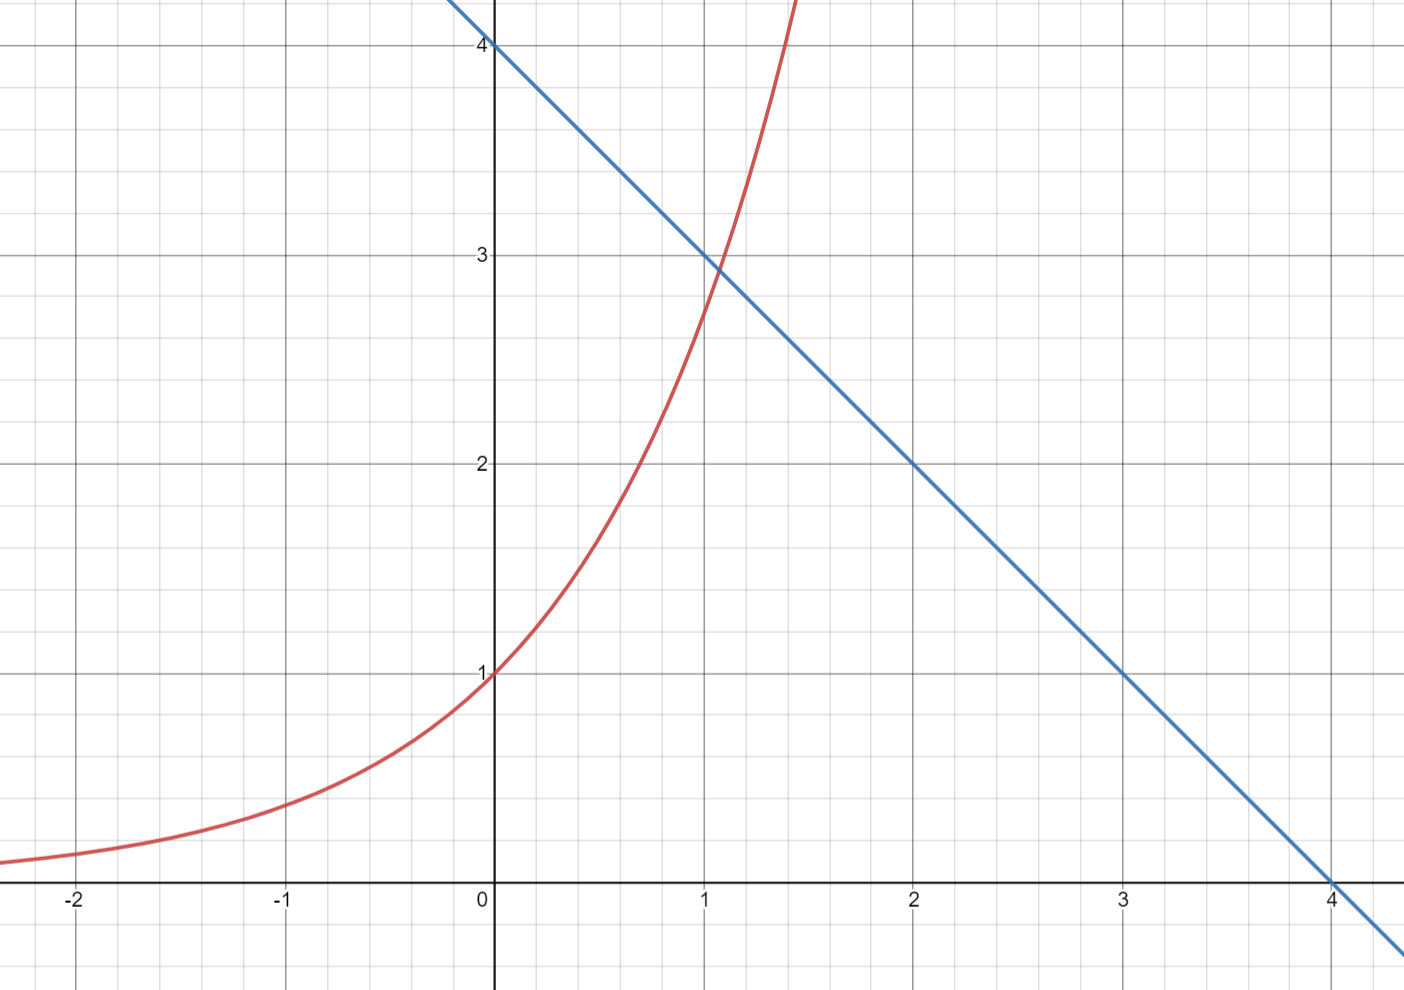
\includegraphics[scale=0.6]{06-Raices/1a.png}
	
	Vemos que se intersecan en el intervalo $[1; 2]$, es decir que existe una raíz en ese intervalo.
	
	\subsection{b}
	$f_2(x)=\sen(x)-2x+1$
	
	$\sen(x)-2x+1=0 \rightarrow \sen(x)=2x-1$
	
	Haciendo el gráfico:
	
	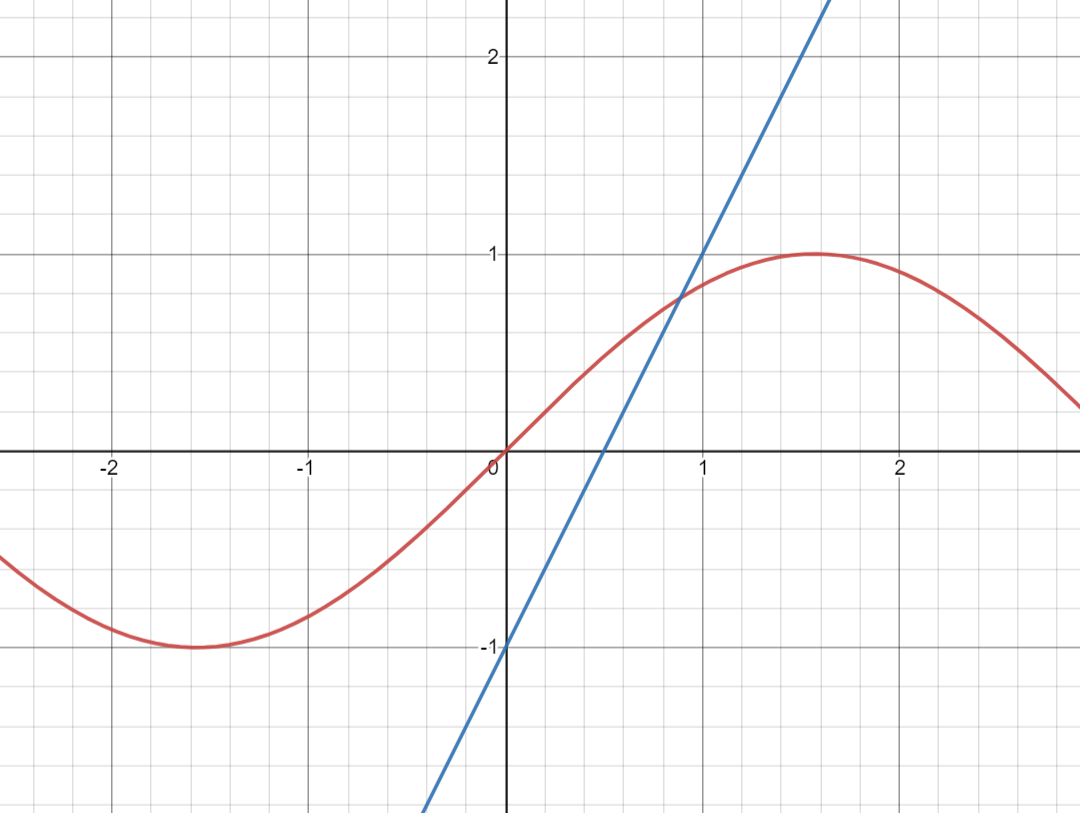
\includegraphics[scale=0.6]{06-Raices/1b.png}
	
	Vemos que tiene una raíz en el $[0; 1]$.
	
	\subsection{j}
	$f_{10}(x)=\ln(x)+x^2-8x+12$
	
	$\ln(x)+x^2-8x+12=0 \rightarrow \ln(x)=-x^2+8x-12$
	
	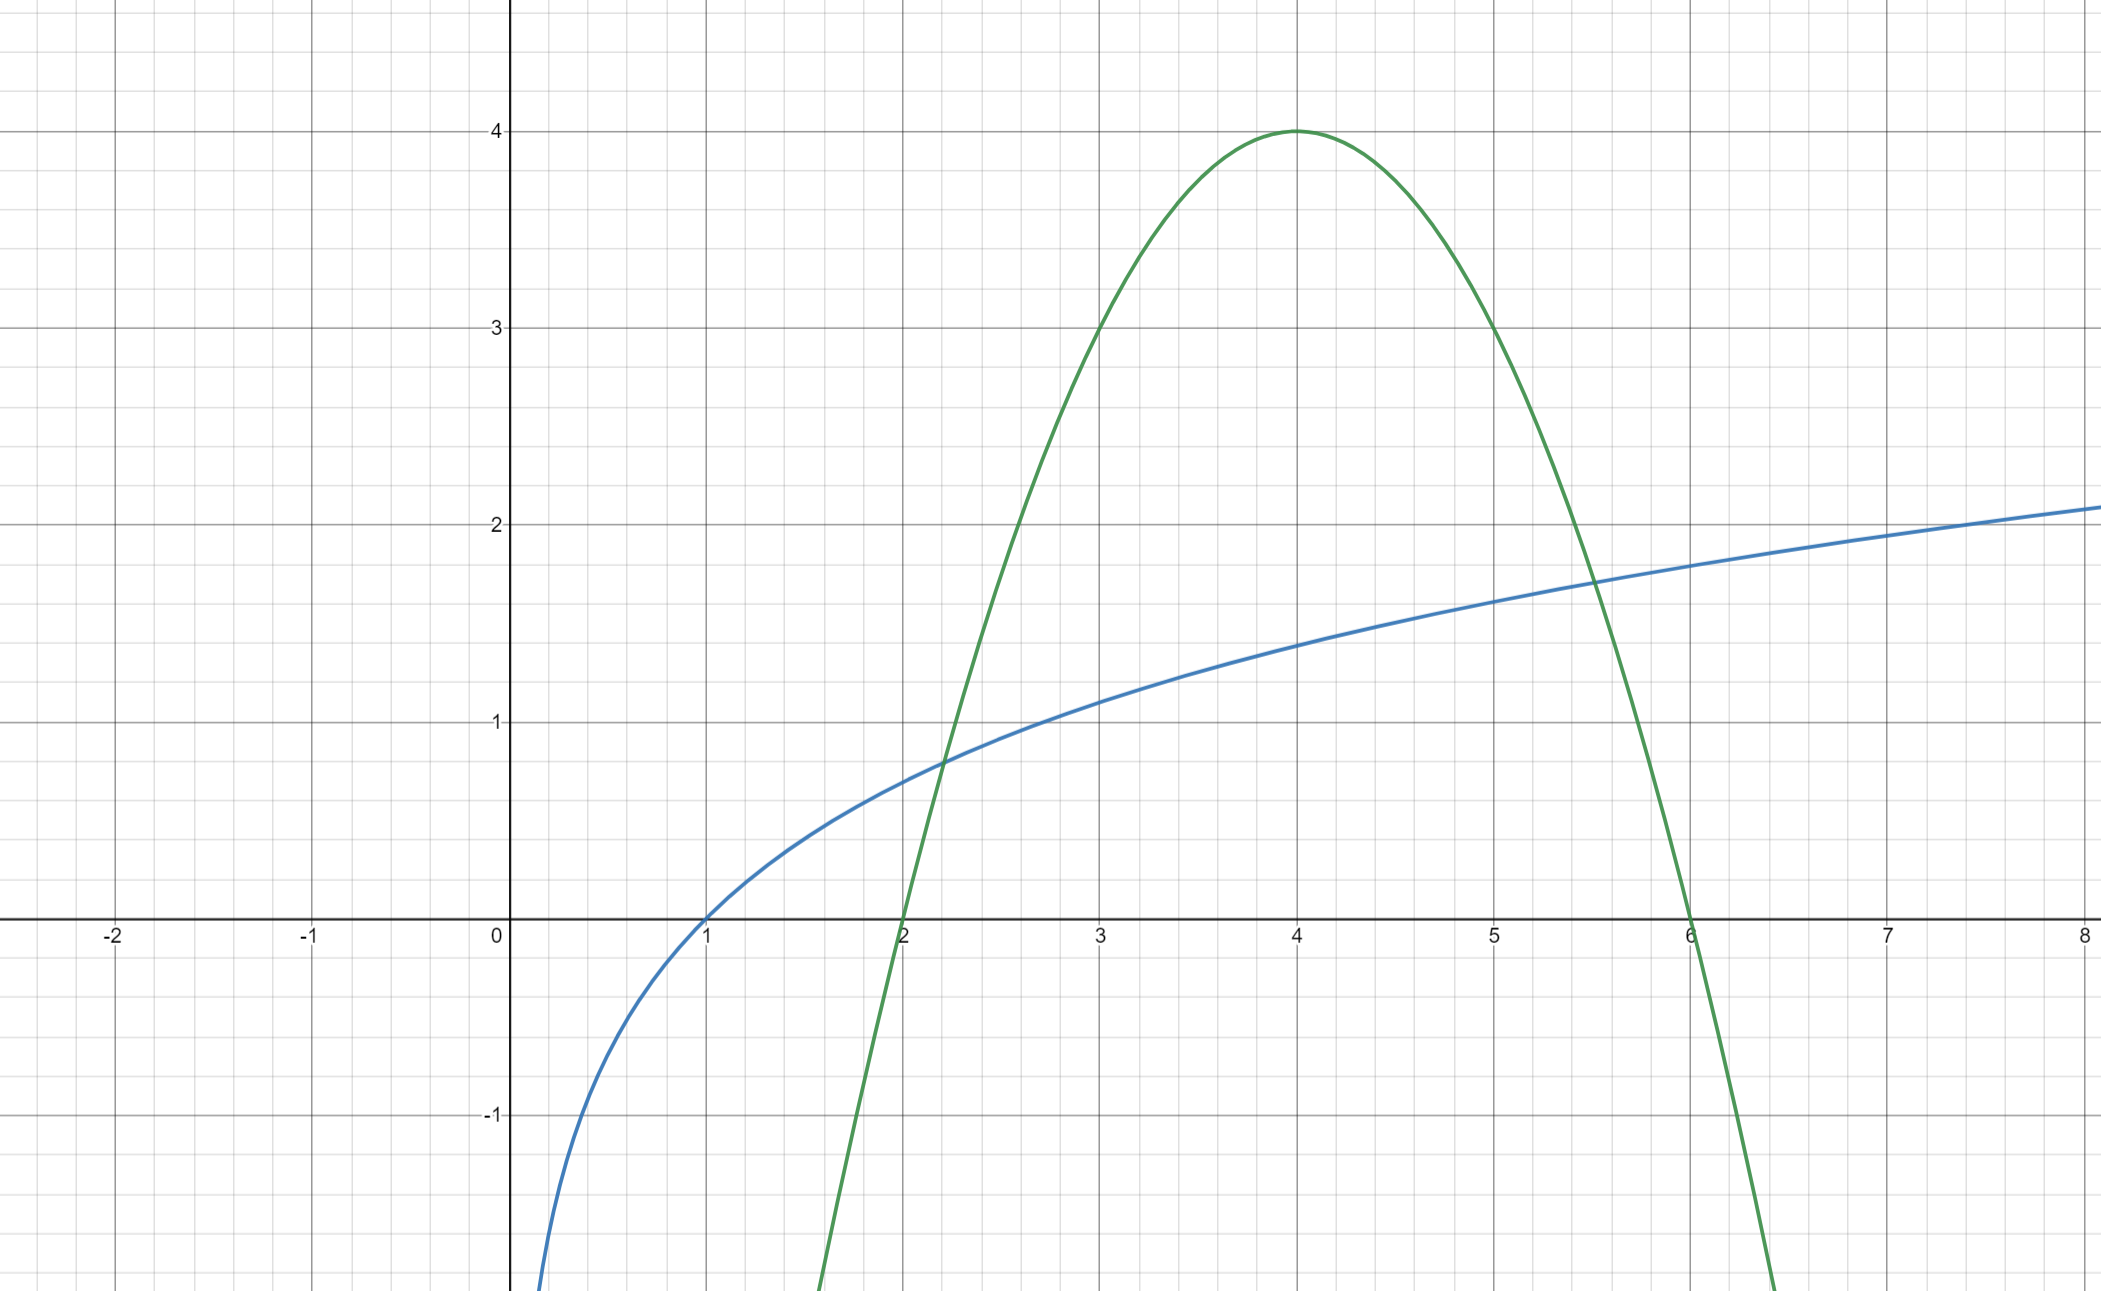
\includegraphics[scale=0.45]{06-Raices/1j.png}
	
	Vemos gracias al gráfico que tenemos 2 raíces una en el $[2; 3]$ y $[5; 6]$
	
	Sin embargo, si hacemos un análisis de las gráficas...: sabemos que la logarítmica se hace asintótica en $x=0$, mientras que la cuadrática tiene dominio en todos los reales, por lo tanto, en \textbf{\underline{ALGÚN}} momento se tienen que cruzar, este cruce se va a dar en el $[0; 1]$. (mostrar gráfica en Desmos).
	
	\subsection{extra, tramposo}
	$f_e(x)=e^x-x^2-4x-2$
	
	$e^x-x^2-4x-2=0 \rightarrow e^x=x^2+4x+2$
	
	Hacemos las gráficas:
	
	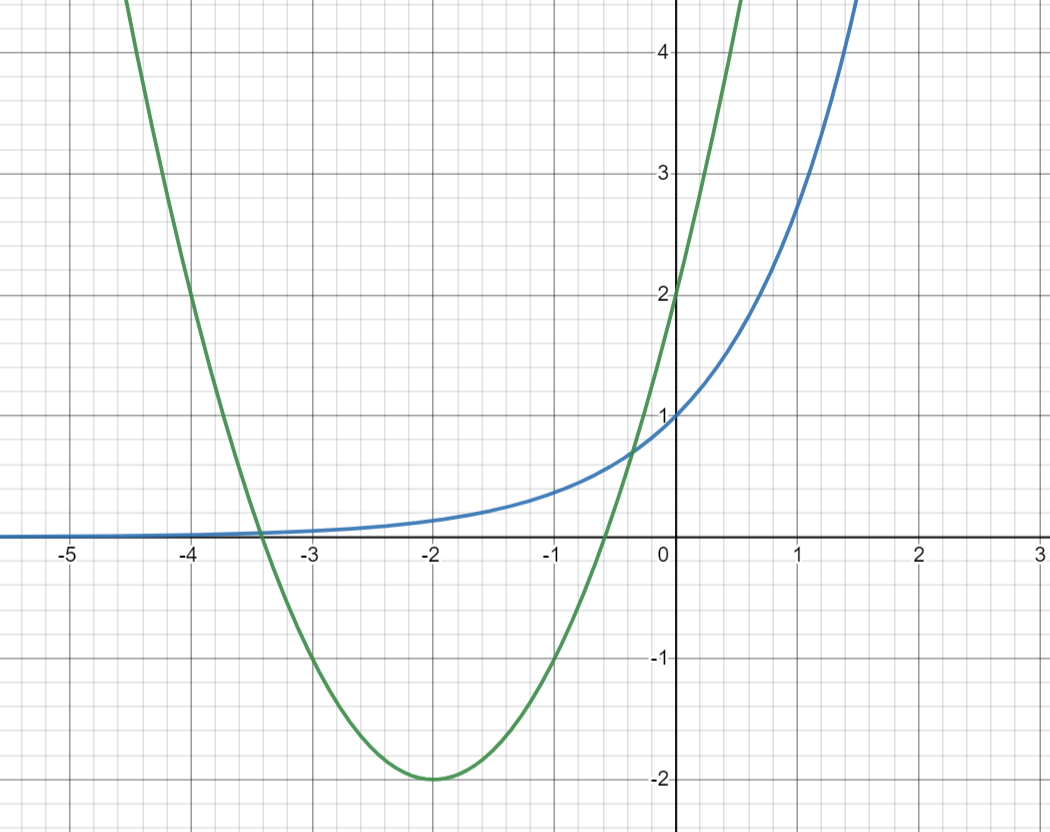
\includegraphics[scale=0.6]{06-Raices/1x.png}
	
	Podemos identificar 2 raíces, una en el $[-4; -3]$ y otra en el $[-1; 0]$
	
	Sin embargo, pasa algo parecido al análisis que hicimos en el ejercicio previo. Vemos que la gráfica de la exponencial quedó por debajo de la cuadrática a partir de la raíz que se encuentra en $[-1; 0]$. Ahora, sabemos que a la larga, una exponencial va a tender a crecer mucho más rápido que la cuadrática, por ende, en algún momento se van a volver a cruzar. Este cruce se da en el $[3; 4]$. Para saber donde se da el cruce, hay que aplicar el teorema de Bolzano e ir evaluando en valores sucesivos, hasta dar con el intervalo que contiene a la raíz. (mostrar gráfico).
	
	Entonces, se concluye con que esta función tiene 3 raíces.
	
	\section{Ejercicio 4 (Bisección)}
	Indique un intervalo para la raíz positiva de $x^2-2x-2=0$. Utilice el método de bisección para calcular la raíz con dos decimales exactos. Establezca el número máximo de pasos necesarios para aproximar la raíz con una precisión de $10^{-6}$.
	
	Para identificar el intervalo, procedemos como el ejercicio 1:
	
	$x^2=2x+2$
	
	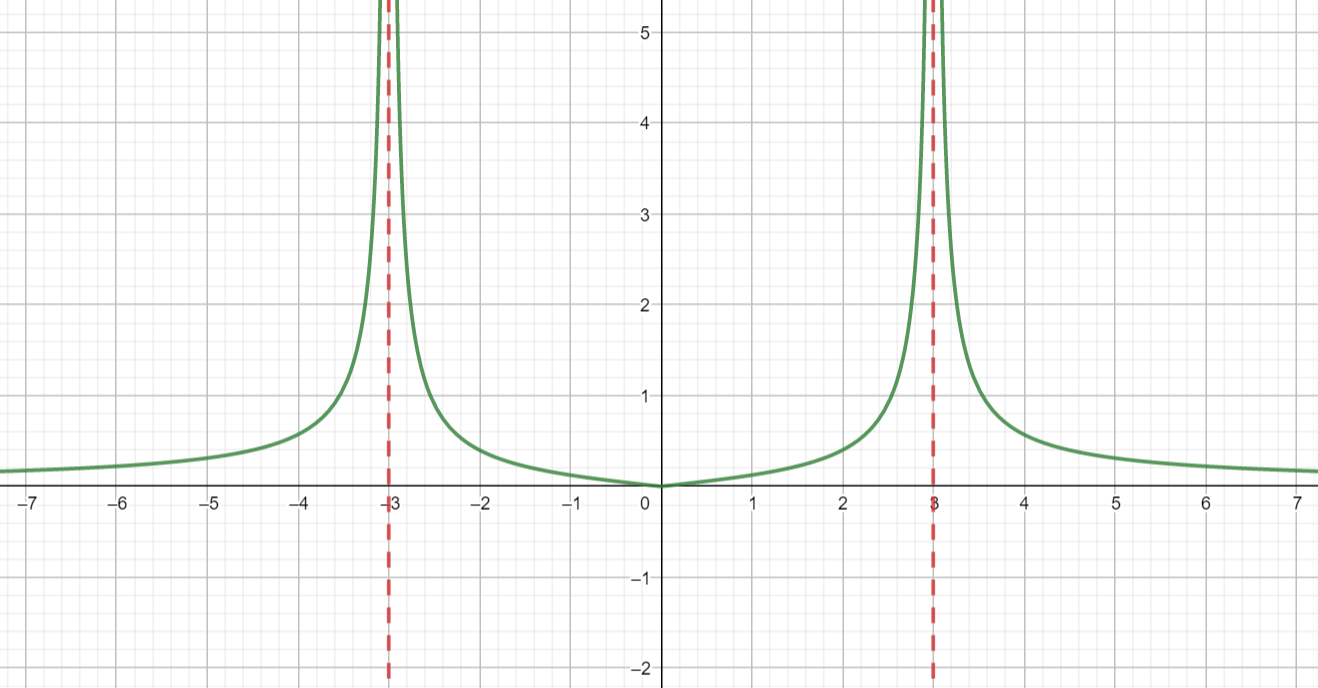
\includegraphics[scale=0.6]{06-Raices/4.png}
	
	Vemos que la raíz se encuentra en el $[2; 3]$.
	
	El cálculo de la raíz lo vemos en un excel ;).
	
	Por último, para el punto que nos piden calcular las iteraciones necesarias para lograr cierta precisión $\varepsilon <10^{-6}$. Esta propiedad es única para este método.
	
	La formulita para calcular es la siguiente:
	
	$\displaystyle \frac{b-a}{2^{i}}<\varepsilon$
	
	Reemplazamos los datos de nuestro ejercicio y despejamos $i$ que es la cantidad de iteraciones.
	
	$\displaystyle \frac{3-2}{2^{i}}<10^{-6} \rightarrow \frac{1}{2^i} <10^{-6} \rightarrow 2^i > 10^6 \rightarrow i\log(2)>6 \rightarrow i > \frac{6}{\log(2)} \rightarrow $ \fcolorbox{black}{yellow}{$i>19.93$}
	
	Como las iteraciones son números enteros siempre tomamos el entero más alto que le sigue, entonces son SUFICIENTES 20 iteraciones.
	
	\textbf{IMPORTANTE:} son iteraciones suficientes porque puede ocurrir que esa precisión se logre antes (por esto último no es condición necesaria).
	
	\section{Ejercicio 5 (Bisección)}
	Cada una de las siguientes funciones verifica que $\text{sg}[f(a)]\neq\text{sg}[f(b)]$ en $(a, b)=(0, 1)$ ¿Qué punto localiza el algoritmo de bisección? ¿Es una raíz? Justifique.
	\subsection{b}
	$f(x)=\cos(10x)$
	
	Vamos a hacer un gráfico de la función (restringida al $(0, 1)$):
	
	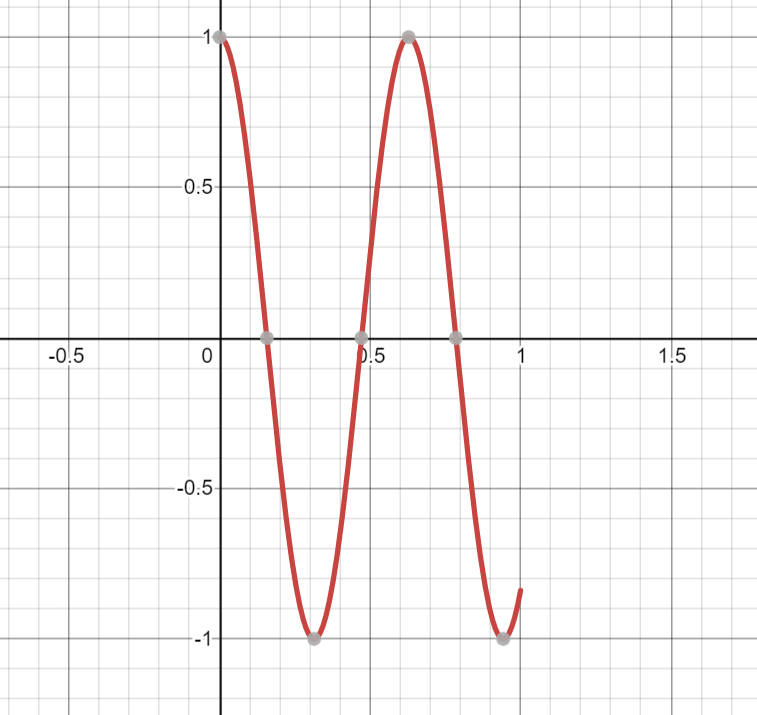
\includegraphics[scale=0.6]{06-Raices/5.png}
	
	Las raíces están en $x=\pi / 20$, $x=3\pi/20$, $x=\pi/4$
	
	Es decir, tenemos 3 raíces en el intervalo, por lo tanto el intervalo estaría mal elegido. Sin embargo, al ir aplicando el algoritmo de bisección converge a una de ellas. En particular, a la raíz ubicada en $x=\pi/4$. Si uno quisiera tener hallar las otras habría que considerar otros intervalos más pequeños, que contengan únicamente a una raíz.
	
	\section{Ejercicio 6 (Bisección)}
	Marque la respuesta correcta y justifique. Para hallar la raíz de una $f(x)$ continua en $(3;5)$ con $\text{sg}[f(3)]\neq \text{sg}[f(5)]$ con $\varepsilon < 10^{-5}$ por Bisección:
	
	El ejercicio se reduce a aplicar la formulita que usamos en el 4.
	
	$\displaystyle \frac{5-3}{2^{i}}<10^{-5} \rightarrow \frac{2}{2^{i}}<10^{-5} \rightarrow \frac{2^{i}}{2}>10^5 \rightarrow 2^{i-1}>10^5 \rightarrow (i-1)\log(2)>5 \rightarrow i > \frac{5}{\log(2)}+1$
	
	\fcolorbox{black}{yellow}{$i>17,61$}
	
	Entonces, como dijimos, siempre se redondea para arriba. Luego, las iteraciones son SUFICIENTES. Recuerden, la precisión que se pide puede llegar a darse antes.
	
	Por lo tanto, son SUFICIENTES 18 iteraciones.
	
	\section{Ejercicio 11 (Regula Falsi)}
	Indique el valor de verdad de las siguientes proposiciones, justificando su respuesta:
	
	a) Sea $e^x+x^4-x-2=0$ con raíz en $(0;1) \implies$ se puede usar Regula Falsi fijando el 1.
	
	Para estos ejercicios de Regula Falsi, debemos calcular la primera y la segunda derivada de la función. Así que primero, debemos escribir la expresión de la función auxiliar (ya que en el enunciado tenemos una ecuación).
	
	$f(x)=e^x+x^4-x-2$
	
	Ahora, se calculan las derivadas:
	
	$f'(x)=e^x+4x^3-1$\\
	$f''(x)=e^x+12x^2$
	
	Las dos son siempre mayores a 0 en ese intervalo. Por ende, ambas tienen signo positivo.
	
	Como $\text{sg}[f']=\text{sg}[f'']$, entonces fijo el extremo b. Es decir, fijo el 1.
	
	Por lo tanto, es \textbf{\underline{VERDADERO}}.\\
	
	b) El método de Bisección siempre converge más lentamente que Regula Falsi.
	
	Esto es \textbf{\underline{FALSO}}. De manera teórica, sabemos que ambas tienen un orden de convergencia igual a 1, entonces para saber quien es más rápido, "desempata" el radio.
	
	Sabemos que el radio de Bisección es fijo $R_B=1/2$, mientras que el radio de Regula Falsi depende del extremo fijado $E$, de la raíz $\alpha$ y de un valor $\varphi \in (a,b)$: $R_{RF}=(\alpha - E) \frac{f''(\varphi)}{2f'(\varphi)}$. Este valor (de forma teórica, ya que casi nunca se puede calcular el radio en forma exacta, sino que se procede a acotarlo) puede ser mayor al radio de Bisección, dando una convergencia más lenta.\\
	
	c) Dada la función $f(x)=x^4-8x^3+30x^2-25x+2-12e^{-x}$, se puede utilizar el Método de Regula Falsi en el intervalo en el intervalo $[1,2]$ fijando el 2.
	
	Calculando las derivadas:
	
	$f'(x)=4x^3-24x^2+60x-25+12e^{-x}$\\
	$f''(x)=12x^2-48x+60-12e^{-x}$
	
	Ambas son siempre positivas en el $[1; 2]$.
	
	Por ende, al tener los signos iguales, se fija el extremo b. Por lo tanto es \textbf{\underline{VERDADERO}}.\\
	
	d) Si $f(x)$ es creciente en $(a,b)$, en el método de Regula Falsi queda fijo el extremo b.
	
	Esto es \textbf{\underline{FALSO}}, ya que además debería ser cóncava hacia arriba, para que la derivada segunda sea también positiva.
	
	\section{Ejercicio 13 (Punto fijo)}
	Indique el valor de verdad de las siguientes proposiciones, justificando su respuesta:
	
	a) Si $0<g'(x)<1$ en el método de Punto Fijo para calcular raíces de ecuaciones entonces la convergencia es en forma de espiral o alternada.
	
	Esto es netamente teórico. Pero si $0<g'(x)<1$ la convergencia es en forma ESCALONADA. Es decir que esto es \textbf{\underline{FALSO}}. Debería ser $-1<g'(x)<0$ para que converja en forma espiralada. \\
	
	b) Sea $e^x+x^4-x-2=0$ con raíz en $(0,1) \implies $ se puede usar $g(x)=e^x+x^4-2$ para hallar la raíz por el método de punto fijo.
	
	Recordar que el objetivo del método de Punto fijo es obtener una expresión $x=g(x)$. Es decir, haciendo algún paso algebraico, hay que despejar una $x$.
	
	Luego $x_{i+1}=g(x_i)$
	
	En este caso, simplemente lo que se hizo es pasar la $x$ de la ecuación al otro lado sumando.
	
	Para \underline{asegurar} la convergencia se deben cumplir:
	
	$\circled{1}$ $|g'(x_i)|<1, \forall x_i \in [a;b]$
	
	$\circled{2}$ $g(x_i) \in (a;b), \forall x_i \in [a;b]$
	
	Vamos a verificar la primera condición:
	
	$g'(x)=e^x+4x^3$
	
	Si analizamos un poco, vamos a ver que no se cumple, ya que siempre $|g'(x)|>1$ en el intervalo $[0;1]$. Por ende no podemos asegurar la convergencia.
	
	Estas dos condiciones son suficientes, no necesarias. Podría ocurrir que converge. (veamos el excel)\\
	
	c) La función $\displaystyle g(x)=\sqrt[3]{2x-1}$ puede utilizarse para hallar una raíz con el método de punto fijo.
	
	El ejercicio no da pistas de intervalos ni una ecuación sobre la cual está basada esta $g$, así que vamos a calcularla nosotros:
	
	Sabemos que si exista una $g$, esta está igualada a $x$, entonces:
	
	$x=\sqrt[3]{2x-1} \rightarrow \sqrt{x^3}=2x-1 \rightarrow x^3-2x+1=0$
	
	Esta ecuación tiene raíces en $x=-1.618033989\dots$, $x=1$, $x=0.6180339887\dots$
	
	Vamos a ver si el método converge para la primera raíz:
	
	Para la primera condición, hallemos $g'(x)$:
	
	$\displaystyle g'(x)=\frac{2}{3}\frac{1}{\sqrt[3]{(2x-1)^2}}$
	
	Consideremos el intervalo $[-2; -1]$ (que contiene a la raíz). La derivada es monótona creciente en este intervalo, y también es continua. Por ende, el valor máximo de la derivada va a estar en $x=-1$
	
	$|g'(-1)|=0.3204999\dots$, por ende la primer condición se cumple.
	
	Veamos la segunda:
	
	$\circled{2}$ $g(x_i) \in (a;b), \forall x_i \in [a;b]$
	
	Como la función $g$ es monótona creciente en el intervalo, podemos probar los extremos del intervalo:
	
	$g(-2)=-1.709975947\dots$, que pertenece a $[-2;-1]$
	
	$g(-1)=-1.44224957$, que también pertenece a $[-2;-1]$
	
	Por ende, ambas condiciones se cumplen, se puede garantizar la convergencia del método.
	
	Por lo tanto, es \textbf{\underline{VERDADERO}}.\\
	
	Sin embargo, ¿qué pasa con las otras raíces?
	
	Si intentamos verificar las condiciones, vamos a ver que no se cumplen. Para el caso de la raíz en $x=1$ si se cumplen, pero depende que intervalo tomemos.
	
	(ir al Excel)
	
	\section{Ejercicio 15 (Punto fijo)}
	
	Dada la ecuación $f(x)=0$ con $\displaystyle f(x)=e^x-\frac{x}{x-1}$. Indique con cual o cuales de las siguientes $g(x)$ converge el método de punto fijo.
	
	Primero que nada, las raíces estarían en $[-1;0]$ y $[1;2]$:
	
	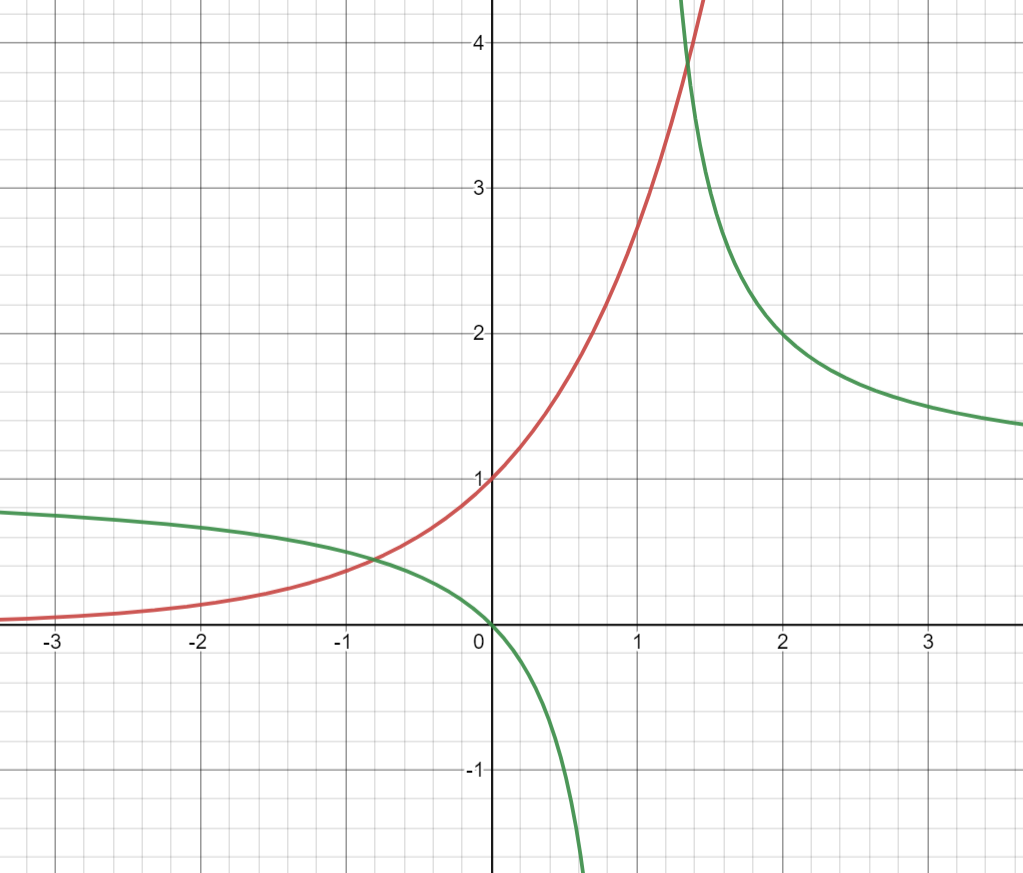
\includegraphics[scale=0.55]{06-Raices/15.png}
	
	Habría que plantear el ejercicio para ambos casos, pero las respuestas de la guía están basadas en la raíz positiva, así que vamos a basar nuestra solución en eso.
	
	a) $g_1(x)=e^x(x-1)$
	
	Calculando la primera derivada: $g'(x)=xe^x$
	
	Esta derivada nunca es menor que uno en el $[1; 2]$, por ende esta $g$ no me sirve, ya que no me asegura la convergencia.\\
	
	b) $\displaystyle g_2(x)=\ln\left(\frac{x}{x-1}\right)$
	
	Sin analizar la derivada, podemos ir por el camino de la segunda condición, buscando un contraejemplo.
	
	Por ejemplo, $\displaystyle g(1.05)=\ln\left(\frac{1.05}{1.05-1}\right)=3.044522\dots \notin (1; 2)$
	
	Por ende, no nos sirve porque no garantiza la convergencia.\\
	
	c) $\displaystyle g_3(x)=\frac{x}{e^x}+1$
	
	Vamos con la primera derivada:
	
	$\displaystyle g'(x)=\frac{e^x-xe^x}{e^{2x}}=\frac{1-x}{e^x}$
	
	De acá podemos razonar:
	
	- El numerador siempre está entre $0$ y $-1$.\\
	- El denominador siempre es mayor a $e^1$
	
	Uniendo estas dos, podemos concluir que $|g'(x)|<1 \forall x \in [1;2]$
	
	Luego, para analizar la segunda condición:
	
	$\displaystyle g(x)=\frac{x}{e^x}+1$, en la fracción siempre vamos a tener un número entre 0 y 1, y luego, sumándole el 1, nos va a terminar quedando siempre un número que esté comprendido entre 1 y 2.
	
	Por ende, se cumple también la segunda condición y podemos garantizar la convergencia.\\
	
	d) $\displaystyle g_4(x)=x-\frac{f(x)}{f'(x)}$

	Es el método de Newton-Raphson, por ende converge.
	
	El método de Newton-Raphson usa la fórmula:
	
	$\displaystyle x_{i+1}=x_i-\frac{f(x_i)}{f'(x_i)}$.
	
	En este método, se intenta buscar que el cociente dé lo más chico posible. Para eso, es conveniente que el numerador sea chico y el denominador sea grande.
	
	Calculemos $\displaystyle f'(x)=e^x+\frac{1}{(x-1)^2}$
	
	Y ahora, pasamos al excel.
	
	\section{Ejercicio 17 (Newton-Raphson)}
	Dada la siguiente ecuación: $x^5-2x^3-\ln(x)=0$ utilice el método de Newton Raphson con $x_0=1$ e itere hasta que se puedan asegurar 5 decimales. ¿Qué ocurre si parte de $x_0=1.1$? Explique.
	
	Para poder aplicar el método, vamos a calcular la derivada:
	
	$\displaystyle f'(x)=5x^4-6x^2-\frac{1}{x}$
	
	Vamos al Excel a ver como converge.
	
	Luego, para el $x_0=1.1$, lo que pasa es que el primer $x$ que obtenemos es un número negativo. Y en la iteración siguiente, cuando queremos hacer $f(x_1)$ no podemos, ya que nos va a quedar un logaritmo con argumento negativo.
	
	\section{Ejercicio 21 (Newton-Raphson)}
	La ecuación $x^4-4x^2+4=0$ tiene una raíz en $x=-\sqrt{2}$. El método de Newtoh-Raphson se acerca a dicha raíz con una precisión de $10^{-9}$ luego de 20 iteraciones. La causa de que la convergencia sea tan lenta se debe a que:
	
	\begin{enumerate}[label=\alph*)]
		\item $f''(x)$ cambia de signo en las proximidades de $x=-\sqrt{2}$
		\item Se consideró un $x_0$ tal que $f(x_0)\bullet f''(x_0)<0$
		\item $x=-\sqrt{2}$ es una raíz con orden de multiplicidad mayor a 1
		\item Ninguna de las causas anteriores es correcta
	\end{enumerate}

	Iremos descartando una por una:
	
	Por la a):
	
	$f'(x)=4x^3-8x$\\
	$f''(x)=12x^2-8$
	
	$f''(x)=0 \rightarrow 12x^2-8=0 \rightarrow x=\pm \sqrt{\frac{2}{3}}\approxeq-0.8164\dots$, que no está próximo a $-\sqrt{2}=-1.41 \dots$
	
	Por ende, esta no es verdadera.
	
	Por la b):
	
	Nos enuncian una de las condiciones suficientes de Fourier, sin embargo en ningún momento nos dan el $x_0$ utilizado, por ende no podemos saber si esto es cierto o no.
	
	Por la c):
	
	Verifiquemos que la multiplicidad de $x=-\sqrt{2}$ es mayor a 1:
	
	$f(-\sqrt{2})=0$\\
	$f'(-\sqrt{2})=0$
	
	Da 0 para la derivada primera también, tiene un orden de multiplicidad mayor a 1.
	
	\textit{Otra forma de darse cuenta es ver que esa función es una \underline{bicuadrada}}, pudiendose factorizar:\\ $f(x)=(x^2-2)^2$
	
	La multiplicidad mayor a 1 es causa de convergencia lenta en el método de Newton-Raphson, por ende esta opción es la \textbf{verdadera}.
	
	Para estos casos hay que usar el método de Newton-Raphson para raíces múltiples.
	
	Si conocemos el orden de multiplicidad de la raíz podemos usar:
	
	$\displaystyle x_{i+1}=x_i-m\frac{f(x_i)}{f'(x_i)}$, con $m$ siendo el orden de multiplicidad.
	
	En cambio, si desconocemos este último, debemos usar el método de Newton-Raphson para raíces múltiples, cuya fórmula es:
	
	$\displaystyle x_{i+1}=x_i-\frac{f(x_i)\cdot f'(x_i)}{[f'(x_i)]^2-f(x_i)\cdot f''(x_i)}$
	
	\section{Ejercicio 26 (Newton-Raphson)}
	Aplique el método de Newton-Raphson a $x^3-2x^2-3x+10=0$ con $x_0=1.9$. ¿Es posible dar una explicación al comportamiento extraño de los valores iterados sucesivos?
	
	Como siempre, vamos a calcular la derivada:
	
	$f'(x)=3x^2-4x-3$
	
	Con esto, vamos al excel
	
	Lo que está pasando es que $x=1.9$ es un valor cercano a un mínimo relativo.
	
	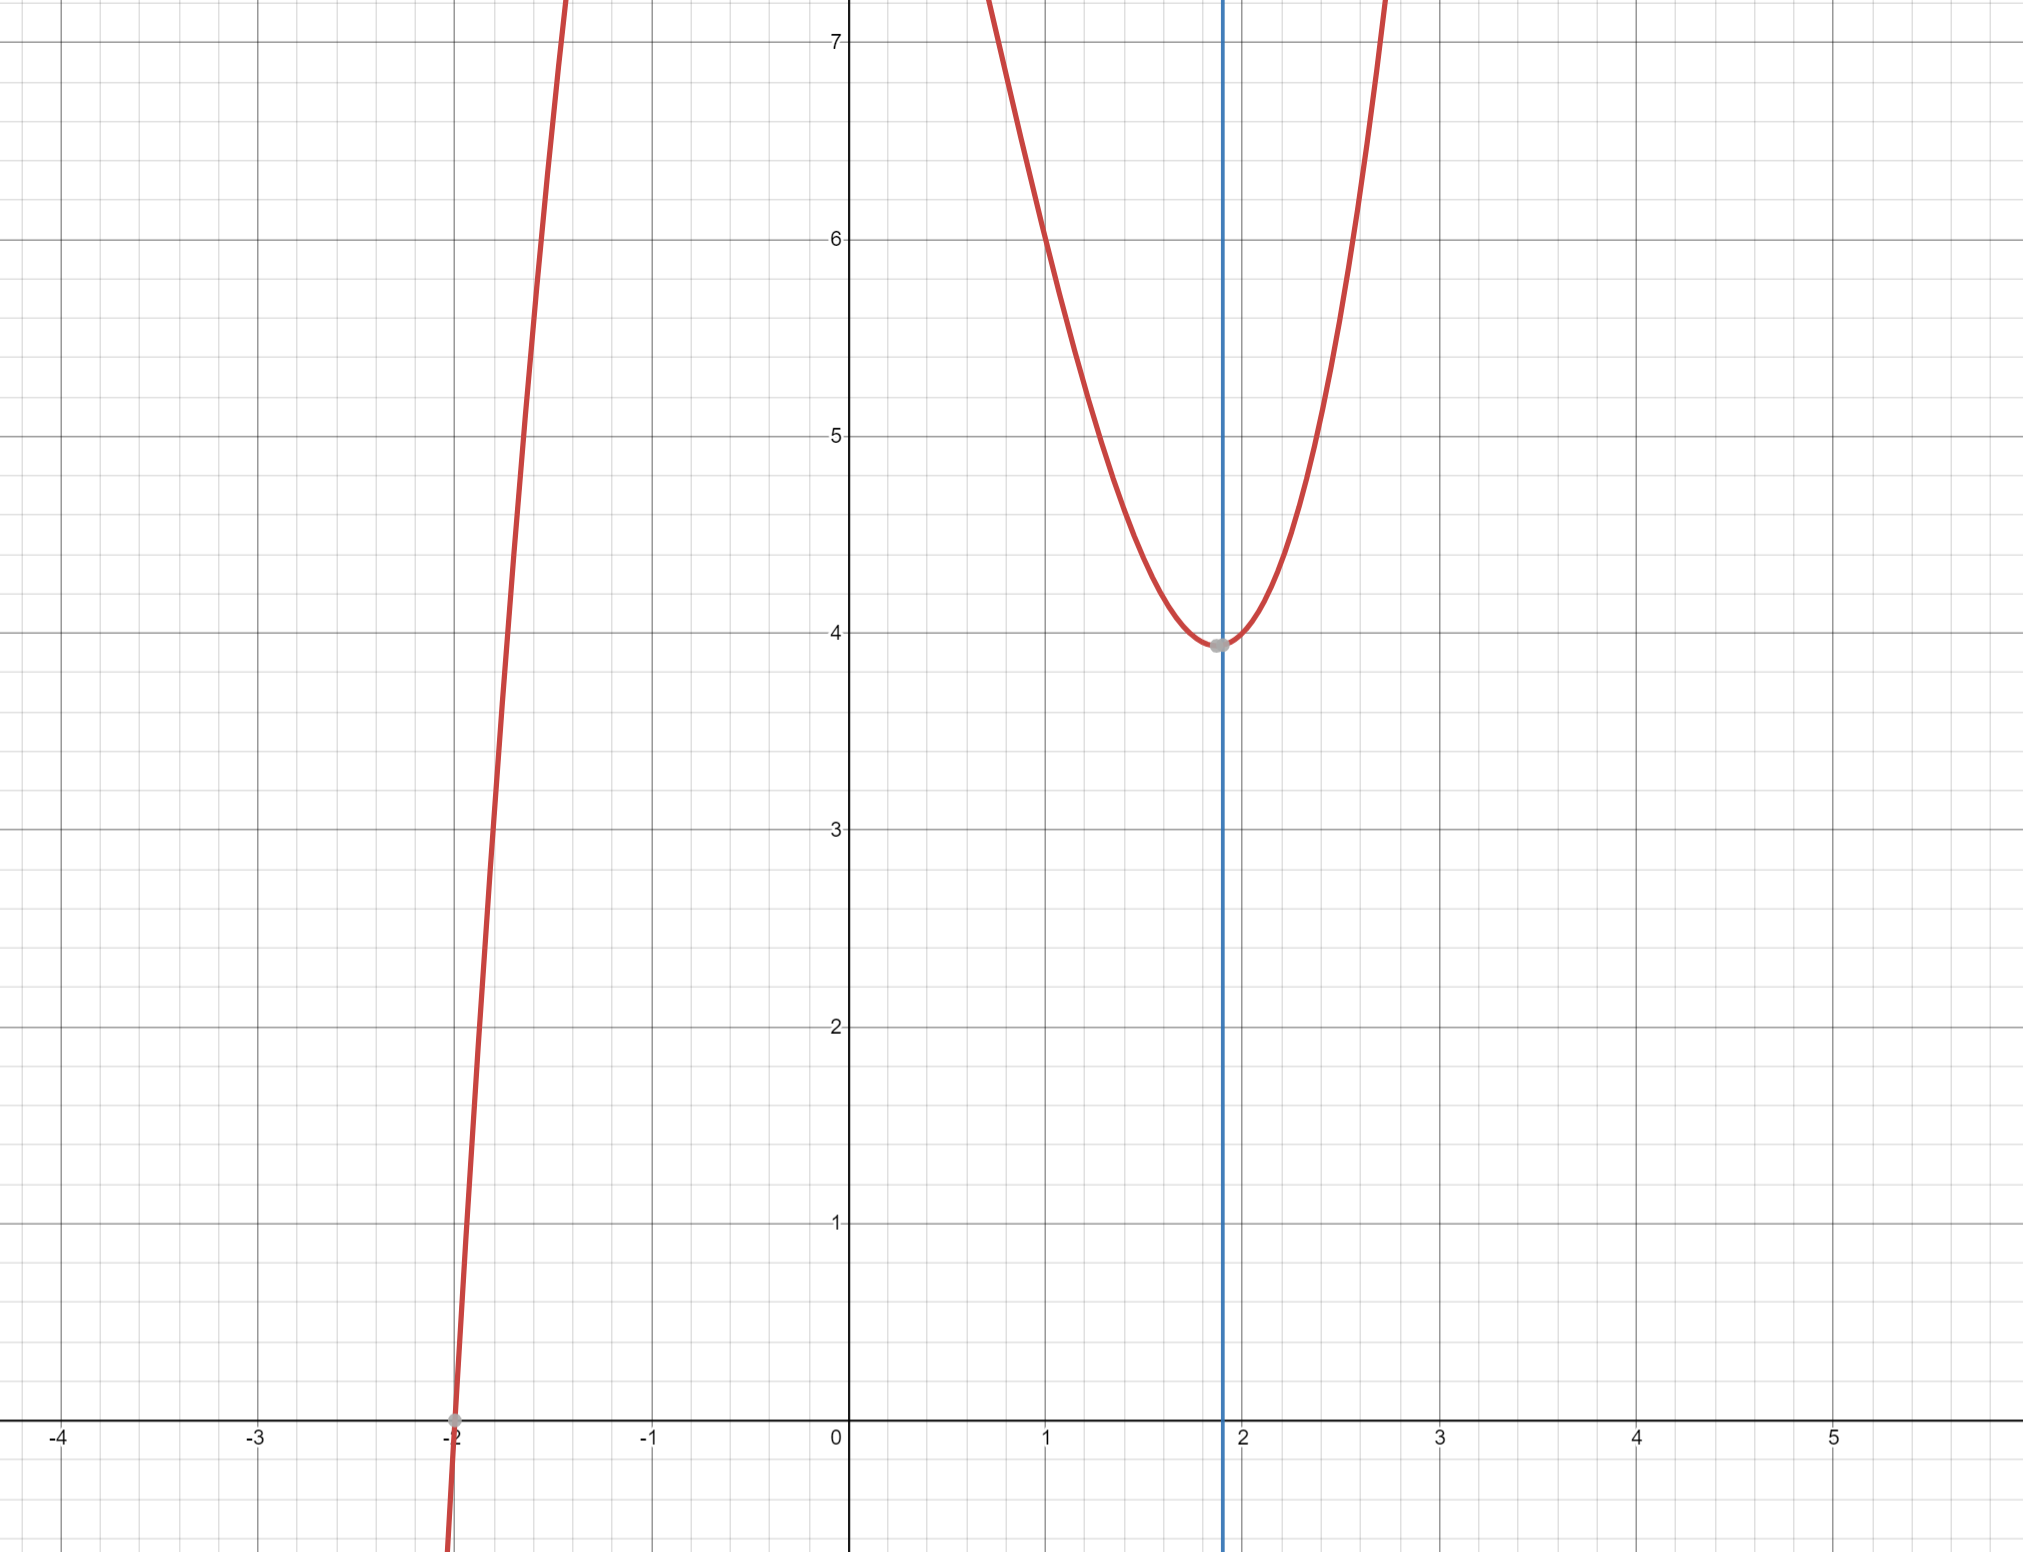
\includegraphics[scale=0.45]{06-Raices/26.png}
	
	\section{Ejercicio 30 (Todos)}
	
	Calcule la raíz cuadrada de 3 con un error menor que $10^{-8}$, utilizando los siguientes métodos:
	
	a) Bisección\\
	b) Punto fijo\\
	c) Regula-Falsi\\
	d) Newton-Raphson
	
	Seleccione un criterio de paro adecuado. Compare la rapidez de convergencia de todos los métodos (indique cuántas iteraciones fueron necesarias en cada uno).\\
	
	Para hallar esa raíz podemos usar la ecuación $x^2-3=0$
	
	Para punto fijo, tener cuidado de no usar el despeje:
	$x^2=3 \rightarrow x=\frac{3}{x}$
	
	Ya que vamos a tener que $x_1=\frac{3}{x_0}$, luego $x_2=\frac{3}{x_1}=\frac{3}{\frac{3}{x_0}}=x_0$, entonces luego $x_3=\frac{3}{x_2}=\frac{3}{x_0}$, es decir, vamos a quedar loopeando y no nos sirve.
	
	Un despeje válido sería usar $x^2=3 \rightarrow x^2+x=3+x \rightarrow x(x+1)=3+x \rightarrow x=\frac{x+3}{x+1}$
	
	(excel)	
	
\end{document}
 